\documentclass{standalone}
\usepackage{tikz}
\usetikzlibrary{patterns, positioning}


\begin{document}
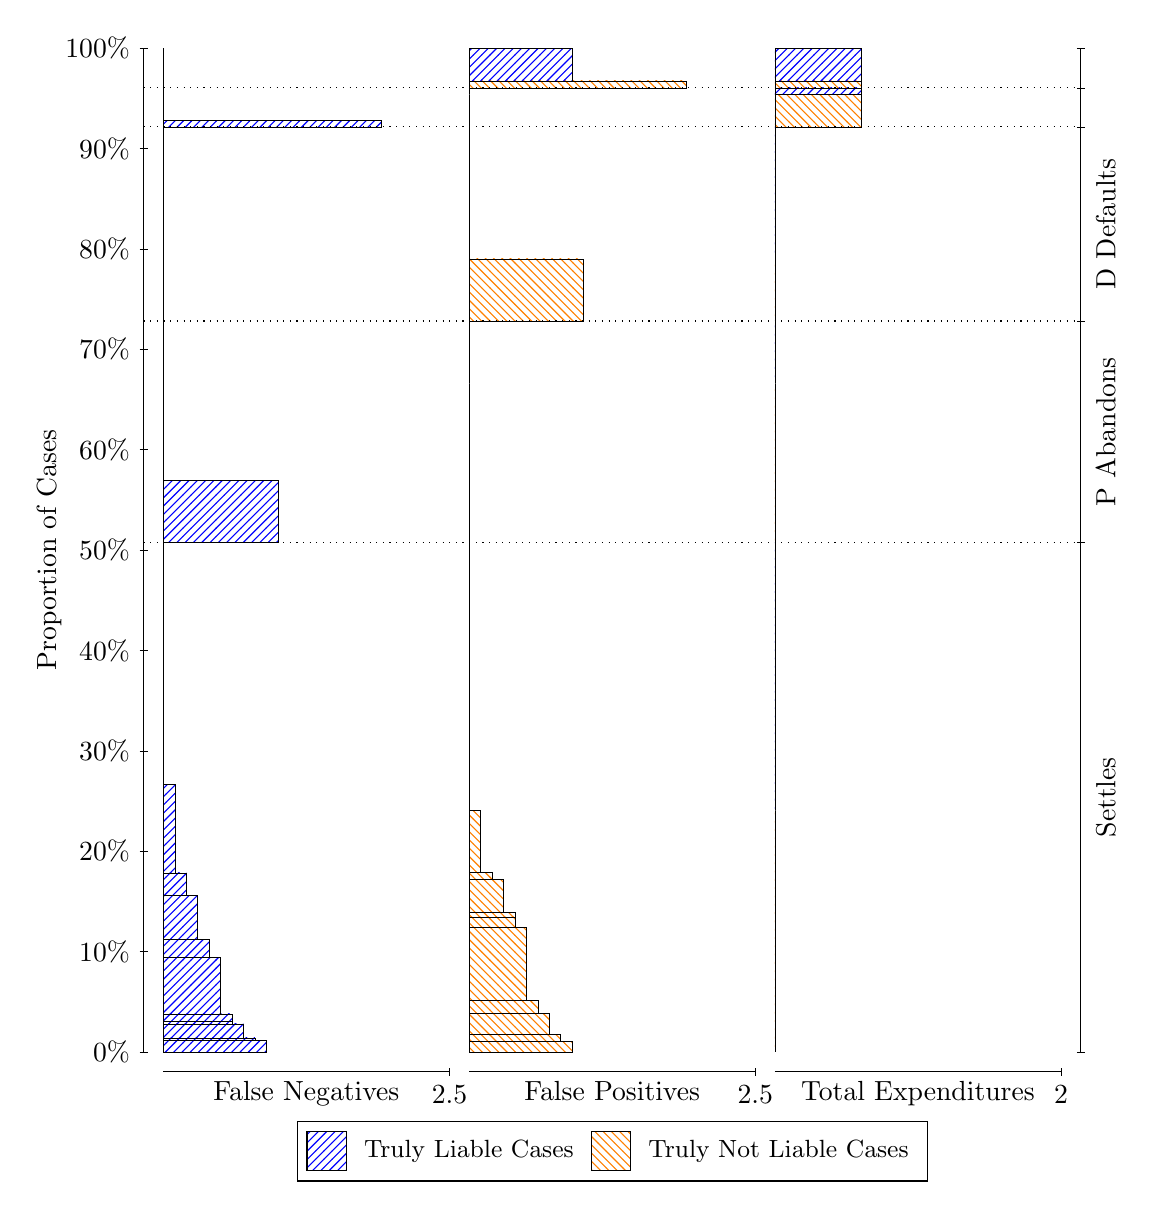
\begin{tikzpicture}
\draw[black, very thin] (1.5,1.75) -- (1.5,14.5);
\node[rotate=90, text=black, anchor=center] at (0.3, 8.125) {Proportion of Cases};
\draw[black, very thin] (1.45,1.75) -- (1.55,1.75);
\node[text=black, anchor=east] at (1.45, 1.75) {0\%};
\draw[black, very thin] (1.45,3.025) -- (1.55,3.025);
\node[text=black, anchor=east] at (1.45, 3.025) {10\%};
\draw[black, very thin] (1.45,4.3) -- (1.55,4.3);
\node[text=black, anchor=east] at (1.45, 4.3) {20\%};
\draw[black, very thin] (1.45,5.575) -- (1.55,5.575);
\node[text=black, anchor=east] at (1.45, 5.575) {30\%};
\draw[black, very thin] (1.45,6.85) -- (1.55,6.85);
\node[text=black, anchor=east] at (1.45, 6.85) {40\%};
\draw[black, very thin] (1.45,8.125) -- (1.55,8.125);
\node[text=black, anchor=east] at (1.45, 8.125) {50\%};
\draw[black, very thin] (1.45,9.4) -- (1.55,9.4);
\node[text=black, anchor=east] at (1.45, 9.4) {60\%};
\draw[black, very thin] (1.45,10.675) -- (1.55,10.675);
\node[text=black, anchor=east] at (1.45, 10.675) {70\%};
\draw[black, very thin] (1.45,11.95) -- (1.55,11.95);
\node[text=black, anchor=east] at (1.45, 11.95) {80\%};
\draw[black, very thin] (1.45,13.225) -- (1.55,13.225);
\node[text=black, anchor=east] at (1.45, 13.225) {90\%};
\draw[black, very thin] (1.45,14.5) -- (1.55,14.5);
\node[text=black, anchor=east] at (1.45, 14.5) {100\%};

\draw[black, very thin] (13.4,1.75) -- (13.4,14.5);
\draw[black, very thin] (13.35,1.75) -- (13.45,1.75);
\node[anchor=west] at (13.35, 1.75) {};
\draw[black, very thin] (13.35,8.2191) -- (13.45,8.2191);
\node[anchor=west] at (13.35, 8.2191) {};
\draw[black, very thin] (13.35,11.033) -- (13.45,11.033);
\node[anchor=west] at (13.35, 11.033) {};
\draw[black, very thin] (13.35,13.498) -- (13.45,13.498);
\node[anchor=west] at (13.35, 13.498) {};
\draw[black, very thin] (13.35,13.995) -- (13.45,13.995);
\node[anchor=west] at (13.35, 13.995) {};
\draw[black, very thin] (13.35,14.5) -- (13.45,14.5);
\node[anchor=west] at (13.35, 14.5) {};

\draw[black, very thin, pattern color=blue, pattern=north east lines] (1.75,1.75) rectangle (3.058,1.899);
\draw[black, very thin, pattern color=blue, pattern=north east lines] (1.75,1.899) rectangle (2.9127,1.9293);
\draw[black, very thin, pattern color=blue, pattern=north east lines] (1.75,1.9293) rectangle (2.7673,2.1056);
\draw[black, very thin, pattern color=blue, pattern=north east lines] (1.75,2.1056) rectangle (2.622,2.1428);
\draw[black, very thin, pattern color=blue, pattern=north east lines] (1.75,2.1428) rectangle (2.622,2.2347);
\draw[black, very thin, pattern color=blue, pattern=north east lines] (1.75,2.2347) rectangle (2.4767,2.9487);
\draw[black, very thin, pattern color=blue, pattern=north east lines] (1.75,2.9487) rectangle (2.3313,3.1826);
\draw[black, very thin, pattern color=blue, pattern=north east lines] (1.75,3.1826) rectangle (2.186,3.7348);
\draw[black, very thin, pattern color=blue, pattern=north east lines] (1.75,3.7348) rectangle (2.0407,4.0256);
\draw[black, very thin, pattern color=blue, pattern=north east lines] (1.75,4.0256) rectangle (1.8953,5.1528);
\draw[black, very thin, pattern color=orange, pattern=north west lines] (1.75,5.1528) rectangle (1.75,8.2191);
\draw[black, very thin, pattern color=blue, pattern=north east lines] (1.75,8.2191) rectangle (3.2033,9.011);
\draw[black, very thin, pattern color=orange, pattern=north west lines] (1.75,9.011) rectangle (1.75,11.033);
\draw[black, very thin, pattern color=orange, pattern=north west lines] (1.75,11.033) rectangle (1.75,11.823);
\draw[black, very thin, pattern color=blue, pattern=north east lines] (1.75,11.823) rectangle (1.75,13.498);
\draw[black, very thin, pattern color=blue, pattern=north east lines] (1.75,13.498) rectangle (4.5113,13.585);
\draw[black, very thin, pattern color=orange, pattern=north west lines] (1.75,13.585) rectangle (1.75,13.995);
\draw[black, very thin, pattern color=orange, pattern=north west lines] (1.75,13.995) rectangle (1.75,14.082);
\draw[black, very thin, pattern color=blue, pattern=north east lines] (1.75,14.082) rectangle (1.75,14.5);
\draw[black, very thin, pattern color=orange, pattern=north west lines] (5.6333,1.75) rectangle (6.9413,1.8873);
\draw[black, very thin, pattern color=orange, pattern=north west lines] (5.6333,1.8873) rectangle (6.796,1.9733);
\draw[black, very thin, pattern color=orange, pattern=north west lines] (5.6333,1.9733) rectangle (6.6507,2.2419);
\draw[black, very thin, pattern color=orange, pattern=north west lines] (5.6333,2.2419) rectangle (6.5053,2.4063);
\draw[black, very thin, pattern color=orange, pattern=north west lines] (5.6333,2.4063) rectangle (6.36,3.3297);
\draw[black, very thin, pattern color=orange, pattern=north west lines] (5.6333,3.3297) rectangle (6.2147,3.467);
\draw[black, very thin, pattern color=orange, pattern=north west lines] (5.6333,3.467) rectangle (6.2147,3.5268);
\draw[black, very thin, pattern color=orange, pattern=north west lines] (5.6333,3.5268) rectangle (6.0693,3.9384);
\draw[black, very thin, pattern color=orange, pattern=north west lines] (5.6333,3.9384) rectangle (5.924,4.0275);
\draw[black, very thin, pattern color=orange, pattern=north west lines] (5.6333,4.0275) rectangle (5.7787,4.8163);
\draw[black, very thin, pattern color=blue, pattern=north east lines] (5.6333,4.8163) rectangle (5.6333,8.2191);
\draw[black, very thin, pattern color=orange, pattern=north west lines] (5.6333,8.2191) rectangle (5.6333,10.241);
\draw[black, very thin, pattern color=blue, pattern=north east lines] (5.6333,10.241) rectangle (5.6333,11.033);
\draw[black, very thin, pattern color=orange, pattern=north west lines] (5.6333,11.033) rectangle (7.0867,11.823);
\draw[black, very thin, pattern color=blue, pattern=north east lines] (5.6333,11.823) rectangle (5.6333,13.498);
\draw[black, very thin, pattern color=orange, pattern=north west lines] (5.6333,13.498) rectangle (5.6333,13.908);
\draw[black, very thin, pattern color=blue, pattern=north east lines] (5.6333,13.908) rectangle (5.6333,13.995);
\draw[black, very thin, pattern color=orange, pattern=north west lines] (5.6333,13.995) rectangle (8.3947,14.082);
\draw[black, very thin, pattern color=blue, pattern=north east lines] (5.6333,14.082) rectangle (6.9413,14.5);
\draw[black, very thin, pattern color=orange, pattern=north west lines] (9.5167,1.75) rectangle (9.5167,4.8163);
\draw[black, very thin, pattern color=blue, pattern=north east lines] (9.5167,4.8163) rectangle (9.5167,8.2191);
\draw[black, very thin, pattern color=orange, pattern=north west lines] (9.5167,8.2191) rectangle (9.5167,10.241);
\draw[black, very thin, pattern color=blue, pattern=north east lines] (9.5167,10.241) rectangle (9.5167,11.033);
\draw[black, very thin, pattern color=orange, pattern=north west lines] (9.5167,11.033) rectangle (9.5167,11.823);
\draw[black, very thin, pattern color=blue, pattern=north east lines] (9.5167,11.823) rectangle (9.5167,13.498);
\draw[black, very thin, pattern color=orange, pattern=north west lines] (9.5167,13.498) rectangle (10.607,13.908);
\draw[black, very thin, pattern color=blue, pattern=north east lines] (9.5167,13.908) rectangle (10.607,13.995);
\draw[black, very thin, pattern color=orange, pattern=north west lines] (9.5167,13.995) rectangle (10.607,14.082);
\draw[black, very thin, pattern color=blue, pattern=north east lines] (9.5167,14.082) rectangle (10.607,14.5);
\draw[black, dotted] (1.5,8.2191) -- (13.4,8.2191);
\draw[black, dotted] (1.5,11.033) -- (13.4,11.033);
\draw[black, dotted] (1.5,13.498) -- (13.4,13.498);
\draw[black, dotted] (1.5,13.995) -- (13.4,13.995);
\draw[black, very thin] (1.75,1.5) -- (5.3833,1.5);
\node[text=black, anchor=north] at (3.5667, 1.5) {False Negatives};
\draw[black, very thin] (5.3833,1.45) -- (5.3833,1.55);
\node[text=black, anchor=north] at (5.3833, 1.45) {2.5};

\draw[black, very thin] (5.6333,1.5) -- (9.2667,1.5);
\node[text=black, anchor=north] at (7.45, 1.5) {False Positives};
\draw[black, very thin] (9.2667,1.45) -- (9.2667,1.55);
\node[text=black, anchor=north] at (9.2667, 1.45) {2.5};

\draw[black, very thin] (9.5167,1.5) -- (13.15,1.5);
\node[text=black, anchor=north] at (11.333, 1.5) {Total Expenditures};
\draw[black, very thin] (13.15,1.45) -- (13.15,1.55);
\node[text=black, anchor=north] at (13.15, 1.45) {2};

\node[text=black, centered, rotate=90] at (13.72, 4.9845) {Settles};
\node[text=black, centered, rotate=90] at (13.72, 9.6261) {P Abandons};
\node[text=black, centered, rotate=90] at (13.72, 12.266) {D Defaults};



\draw (7.449999999999999,1.5) node[draw=none] (baseCoordinate) {};
\begin{scope}[align=center]
        \matrix[scale=0.5, draw=black, below=0.5cm of baseCoordinate, nodes={draw}, column sep=0.1cm]{
            \node[rectangle, draw, minimum width=0.5cm, minimum height=0.5cm, pattern color=blue, pattern=north east lines] {}; &
            \node[draw=none, font=\small, text=black] (B) {Truly Liable Cases}; &
            \node[rectangle, draw, minimum width=0.5cm, minimum height=0.5cm, pattern color=orange, pattern=north west lines] {}; &
            \node[draw=none, font=\small, text=black] (B) {Truly Not Liable Cases}; \\
            };
\end{scope}

\end{tikzpicture}
\end{document}